\chapter{Testing}
There are various types of testing, depending on what is their purpose.

\begin{enumerate}
   \item \textbf{Functional} Testing:
   test that the functionalities of the system work as expected and to discover eventual bugs
   \item \textbf{User} Testing:
   Test that the product is useful to and usable by end users
   \begin{enumerate}
      \item 
      \textit{Alpha} $\longrightarrow$ \textit{"Do you really want these features?"}
      \textit{Beta} $\longrightarrow$ Early version of product distributed to users to check product usability and effective interoperability
   \end{enumerate}
   \item \textbf{Performance} and \textbf{load} testing:
   Test that system \textbf{responds quickly} to service requests and it can handle different loads and \textbf{scales} gracefully as the load increases
   \item \textbf{Security} testing:
   Find vulnerabilities that attackers may exploit
\end{enumerate}

There are two main things to remember when talking about testing,
the first is an old known quote from Dijkstra:
\begin{center}
   \textit{"Program testing can be used to show the \textbf{presence} of bugs, but \underline{never} to show their \textbf{absence}"}
   \note{Edsger W. Dijkstra}
\end{center}

The other is that software \textbf{testing} \textit{\underline{it \textbf{not} equal to}} software \textbf{verification},
which instead involves representing the software in a model to prove some properties.

\section{Functional testing}
The first thing to address is testing \textbf{coverage}:
all code should be executed at least once by the test suite.

Testing \underline{should}\footnote{Actually, finding someone who starts testing on day 0 {--}or even day 100{--} is pretty hard.} start on the day you start writing code, and should possibly be automated, to considerably simplify the \textbf{develop/test cycle} and to allow functional testing to be a staged activity.

\subsection{Unit Testing}
\textbf{Unit testing} consists in testing program units (e.g. function, method) in isolation.

\begin{theorem}[Unit testing principle]
   \label{theo:unit_principle}
If a program unit behaves as expected for a set of inputs that have some shared
characteristics, it will behave in the same way for a larger set whose members share
these characteristics.

\end{theorem}
\note{
   For example:\\
   If your program behaves correctly on the input set ${1, 5, 17, 45, 99}$, you may
   conclude that it will also process all other integers in the range 1 to 99 correctly
}

To exploit the unit testing principle \ref{theo:unit_principle} it is crucial to
identify \textbf{equivalence partitions} i.e. sets of inputs that will be treated the same in your code;
they allow to test a program using several inputs from each equivalence partition.
Besides, keep in mind that programmers make mistakes at \textbf{boundaries}: 
identify equivalence partition and their boundaries and choose inputs at these boundaries.

\subsection{Feature testing}

\section{System and Release testing}
Aside from single functionalities, the system should be tested \textit{as a whole};
to achieve so it is recommended to use a set of scenarios/user stories to identify users’ end-to-end pathways,
to consider the whole system.\\
This is necessary for several reasons:
\begin{enumerate}
   \item To discover \textbf{unexpected/unwanted interactions} between the features
   \item To discover if system features work together effectively to support what
   users really want to do
   \item To make sure system operates as expected in the \textbf{different environments}
   where it will be used
   \item To test \textit{responsiveness}, \textit{throughput}, \textit{security}, and other \textbf{quality} attributes
\end{enumerate}

\textbf{Release testing} instead addresses testing of a system intended to be released to customers,
performing tests in the real operational environment, rather than
in the test one.\\
The aim of is to decide if the system is \textit{good enough} to \textbf{release}, \textit{not} to detect bugs in the system.

Preparing a system for release involves \textbf{packaging} the system for
deployment, installing used software and libraries, configure parameters;
many  mistakes can be made in such process, creating the need for release testing.
\note{
   If you deploy on the cloud, an automated continuous release process can be used.
}

\section{Test Automation}
\textbf{Automated testing} is widely used in \textit{product development} companies.
To facilitate the task there are many testing frameworks available for all widely used programming languages.\\
Executable tests check that software return expected result for input data.

A good practice is to \textbf{structure} automated tests in three parts:
\begin{enumerate}
   \item \textbf{Arrange}\\
   Set up the system to run the test, i.e. define test parameters, mock objects, etc.
   \item \textbf{Action}\\
   Call the unit that is being tested with the test parameters.
   \item \textbf{Assert}\\
   Assert what should hold if test executed successfully.
\end{enumerate}

\begin{lstlisting}
   #Arrange - set up the test parameters
   p=0
   r=3
   n= 31
   result_should_be = 0
   #Action - Call the method to be tested interest = interest_calculator (p, r, n)  #Assert - test what should be true self.assertEqual (result_should_be, interest)
\end{lstlisting}

Note that \textit{test code} can include \textbf{bugs}!
To avoid this tests should be made as simple as possible and they should be reviewed along with the code that they test.

\textbf{Unit tests} are the easiest to automate, and if properly done
can reduce (not eliminate) the need for feature tests.

\texttt{GUI}-based testing expensive to automate, since they multiple assertions are needed to check that a feature has executed as expected; API-based testing is preferrable from this point-of-view.

\textbf{System testing} involves testing system as a \textit{"surrogate user"}, performing  sequences of user actions.
\textit{Manual} system testing is definitely \textbf{boring} and error prone,
so in general should be avoided in favor of testing tools that record a series of actions and \textbf{automatically replay} them.

\section{Test-driven development}
\begin{figure}[htbp]
   \centering
   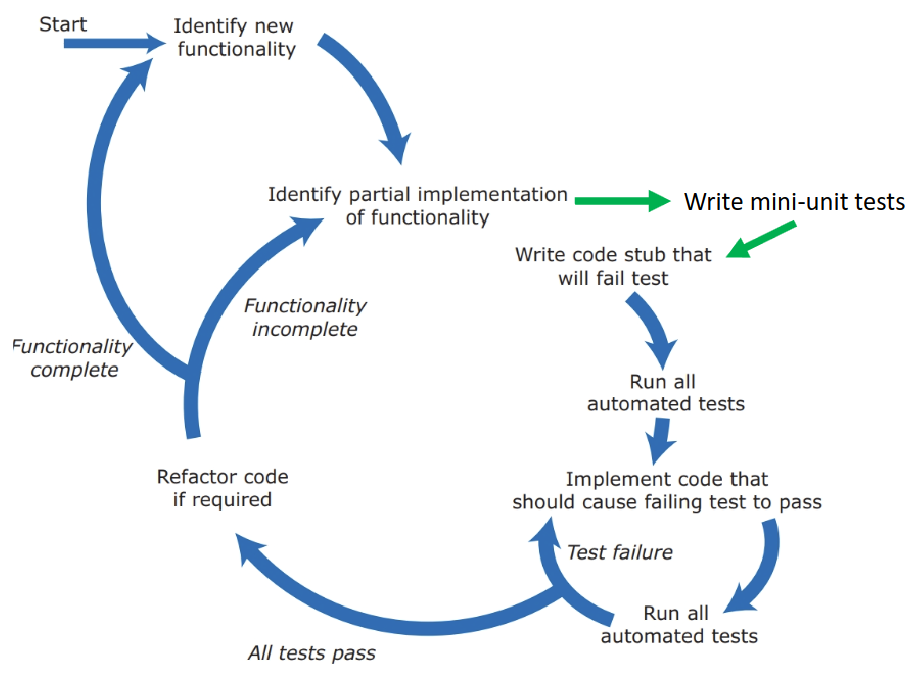
\includegraphics{images/testdriven.png}
   \caption{Test-driven development schema}
   \label{fig:testdriven}
\end{figure}

\begin{theorem}[Extreme Programming]
\textit{"First write executable test, then write the code"}
\end{theorem}

\labelitemize{\textit{Pros}}{
   \begin{enumerate}
      \color{darkgreen}
      \item By exploiting such systematic approach, tests are clearly
      \textbf{linked} to code sections,
      almost eliminating the chance to have untested snippets.
      \item Tests help understanding program
      code
      \item Simplified, incremental debugging
      \item (Arguably) simpler code
   \end{enumerate}
}

\labelitemize{\textit{Cons}}{
\begin{enumerate}
   \color{darkred}
   \item Difficult to apply TDD to system
   testing
   \item TDD \textit{discourages} radical program
   changes
   \item TDD leads you to focus on the tests
   rather than on the problem you are
   trying to solve
   \item TDD leads you to think too much
   about implementation details
   rather than on overall program
   structure
   \item Hard to write "bad data" tests
\end{enumerate}
}

\section{Security Testing}
The two main objectives of \textbf{security testing} are finding \textit{vulnerabilities} exploitable by attackers and providing convincing evidence that the system is sufficiently \textit{secure}.

Finding vulnerabilities is harder than finding bugs, because it implies testing for something that software should \textit{not} do,
thus having a potentially infinite
number of tests.\\
Normal functional tests may not reveal vulnerabilities, besides
the \textbf{software stack} (OS, libraries, dbs, ...) on which your product depends may contain vulnerabilities,
and some of these may arise in the composition of these components.


Comprehensive security testing requires
\textbf{specialist knowledge} and typically implies a risk-based approach:
\begin{enumerate}
   \item identify main security \textbf{risks} to your
   product
   \item develop tests to demonstrate that the
   product \textbf{protects} itself from these risks
\end{enumerate}
When testing security, you need to think like an \textit{attacker} rather than a normal end-user.\\
While it is generally possible to \textit{automate} some of these tests,
others inevitably require manual checking
of behaviour/files.

\section{Limitations of testing}
\begin{enumerate}
   \item You test code against your understanding of what that code
   should do;
   so if you have misunderstood the \textbf{purpose} of the code,
   then this will affect both the code and the tests.
   \item Testing may not provide \textbf{coverage} of all the code you have
   written. 
   \note{
      \textit{Test-Driven development} shifts the problem to code \textbf{incompleteness}.
   }
   \item Testing does \textit{not} really tell you anything about some attributes
   of a program e.g. \textit{readability}, \textit{structure}, \textit{evolvability}...
\end{enumerate}

Often a single \textbf{code reviewer} is used, 
they may be part of same \textit{DevOps} team, but not necessarily.
The reviewer can also comment on \textit{readability} and \textit{understandability} of code, which are aspects that testing cannot address.

A single review session should focus on $200-400$ lines of code, and typically implies using checklist, e.g.
\labelitemize{\footnotesize \textit{Checklist e.g.}}{
   \begin{enumerate}
      \footnotesize
      \item Are meaningful variables and function names used? (\textit{General})
      \item Have all data errors been considered and tests developed for these? (\textit{General})
      \item Are all exceptions explicitly handled? (\textit{General})
      \item Are default function parameters used? (\texttt{Python})
      \item Are types used consistently? (\texttt{Python})
      \item Is the indentation level correct? (\texttt{Python})
   \end{enumerate}
}

Reviews can be "triggered" by commits on shared repositories, and can be eased up by
\textbf{code review tools}, eventually paired with messaging systems like \textit{Slack}.

\begin{figure}[htbp]
   \centering
   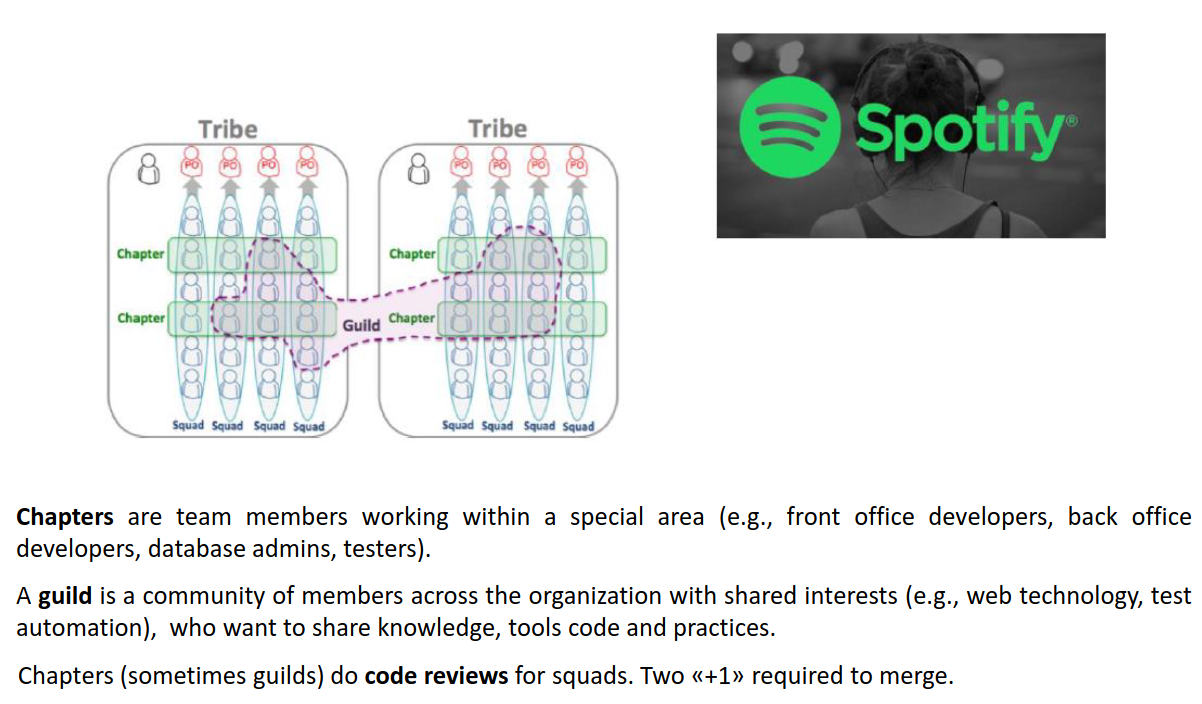
\includegraphics{images/testing_spotify.png}
   \caption{Testing in Spotify}
   \label{fig:testing_spotify}
\end{figure}
\section{Takeaway quotes}
\begin{center}
   \textit{"Pay attention to zeros. If there is a zero, someone will divide by it."}

   \textit{"Testers don’t break software, software is already broken."}
\end{center}